\documentclass{report}
\usepackage{graphicx} % Required for inserting images
\usepackage[italian]{babel}
\usepackage{tikz}
\usepackage{hyperref}
\usepackage{amsmath}
\usepackage{xcolor}

\definecolor{darkgreen}{rgb}{0.0, 0.5, 0.0} % RGB per un verde scuro


\title{Privacy nella Pubblicazione di Dati}
\date{Parte I}

\begin{document}

\maketitle

\tableofcontents

\newpage
Una continua crescita riguardante:
\begin{itemize}
    \item database governativi e aziendali
    \item contenuti generati dagli utenti 
    \item informazioni personali identificative collezioante quando un utente crea un account, scarica un'applicazione, \dots
\end{itemize}
La condivisione dei dati serve per:
\begin{itemize}
    \item studiare le tendenze e fare inferenze statistiche
    \item condividere conoscenza
    \item accedere ai servizi online
\end{itemize}
C'è inoltre l'archiviazione e il calcolo esterno (cloud), che offorno:
\begin{itemize}
    \item risparmio sui costi e benefici dei servizi
    \item maggiore disponibilità e protezione da eventuali disastri
\end{itemize}

\textbf{Per questa serie di motivazioni è fondamentale garantire che la privacy e l’integrità dei dati siano
adeguatamente protette.}

\chapter{Privacy nella Pubblicazione dei Dati}

Quando si parla del rilascio di informazioni per scopi statistici,
è possibile fare una distinzione tra:
\begin{itemize}
    \item \textbf{statistical DBMS:} c'è un'interazione tra client e DBMS, con quest'ultimo che risponde a delle query. Richiede un \textbf{controllo a runtime} delle informazioni rilasciate.
    \item \textbf{statistical data:} non c'è un'interazione; il controllo viene fatto prima del rilascio dei dati, tramite delle autorità competenti
\end{itemize}

\section{Macrodata, microdata, disclosure}
Per \textbf{macrodata} si intendono dati aggregati; le tabelle possono essere classificate in due gruppi:
\begin{itemize}
    \item \textbf{Conteggio/Frequenza:} ogni cella contiene il numero o la percentuali di rispondenti che hanno lo stesso valore per gli attributi considerati.
    Mostrano il numero di volte che un valore compare nei dati (quanti studenti hanno preso un certo voto).
    \item \textbf{Magnitudo:} ogni cella contiene un valore di una \textit{quantità di interesse}. 
    Riportano la somma o media di un valore numerico associato a una cateogoria (somma degli stipendi per dipartimento). 
\end{itemize}

Per \textbf{microdata} si intendono dati non aggregati, ovvero dati specifici e individuali; questo 
tipo di dati sono soggetti a un maggiore rischio di violazione della privacy (attacchi di collegamento).

\subsubsection{Rilascio di informazioni}
Il rilascio di informazioni si riferisce all'\textbf{attribuzione di informazioni sensibili a un rispondente}.

Si può fare una distinzione tra:
\begin{itemize}
    \item \textbf{Identity disclosure:} è quando un terzo può \textbf{identificare} un rispondente tramite le informazioni rilasciate; è un problema
    quando si tratta di microdata, dato che i dati sono dettagliati 
    \item \textbf{Attribute disclosure:} è quando \textbf{informazioni confidenziali} di un rispondente sono 
    rilasciate o possono essere a lui attribuite, con esattezza o con un grado di precisione inferiore a quello atteso 
    \item \textbf{Inferential disclosure:} è quando informazioni sensibili vengono \textbf{dedotte con alta certezza dalle proprietà statistiche dei dati rilasciati}.
\end{itemize}

\subsubsection{Tecniche di protezione per macrodata}
\begin{itemize}
    \item \textbf{Sampling:} pubblicare solo una porzione della popolazione totale; deve essere rappresentativo e privo di bias
    \item \textbf{Special rules:} si definiscono delle restrizioni sul livello di dettaglio che può essere fornito (ad esempio, non pubblicare o rendere
    deducibili i redditi sotto un intervallo di 1000\$)
    \item \textbf{Threshold rules:} definire una cella come sensibile se il numero di rispondenti è inferiore a un soglia
\end{itemize}

\subsubsection{Tecniche di protezione per microdata}
\begin{itemize}
    \item \textbf{Masking:} si trasforma il dataset non rilasciando o modificando i suoi valori. Possono essere:
    \begin{itemize}
        \item \textit{non-perturbative:} il dataset non viene modificato, ma alcuni dati sono soppressi o alcuni dettagli rimossi (sampling, generalizzazione)
        \item \textit{perturbative:} il dataset viene modificato (arrotondamento, \\swapping); viene introdotto del rumore
    \end{itemize}
    \item \textbf{Dati sintetici:} vengono usati dati plausibili ma sintetici;
    \begin{itemize}
        \item \textit{fully synthetic:} il dataset contiene solo dati sintetici
        \item \textit{partially synthetic:} il dataset contiene sia dati sintetici che dati originali
    \end{itemize}
\end{itemize}

\newpage
\subsection{Anonimity problem}
È in continua crescita il numero di record che contengono dati sensibili dei cittadini. Questi record
vengono \textit{de-identificati} prima della loro pubblicazione; tuttavia, questo \textbf{non è sufficiente}: possono essere 
usati altri dati per fare dei collegamenti tra identità de-identificate, facendo dunque
una \textbf{re-identificazione}.

\subsubsection{Esempio}
\begin{figure}[ht]
    \centering
    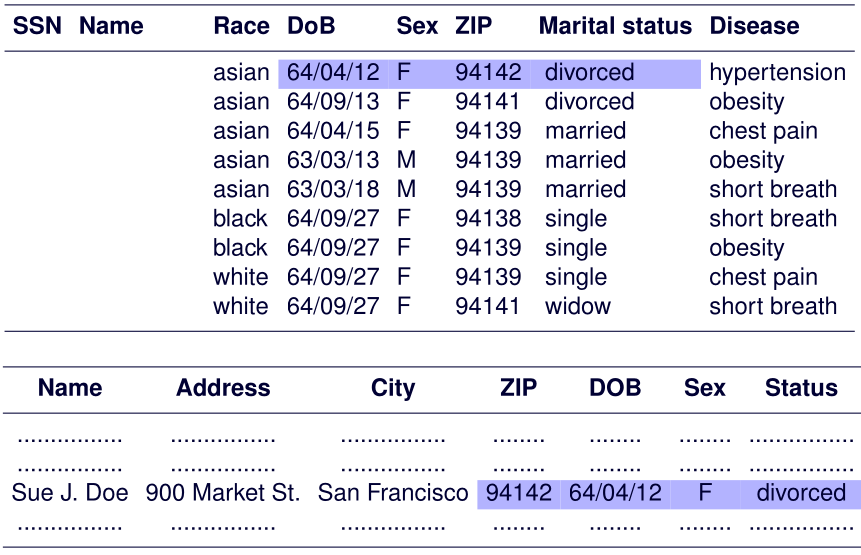
\includegraphics[width=0.9\linewidth]{images/anon-1.png}
\end{figure}
\begin{figure}[ht]
    \centering
    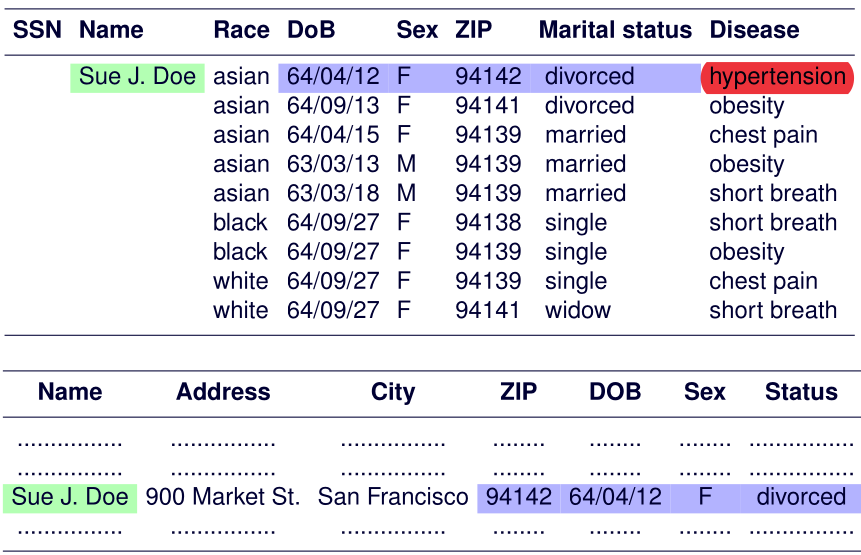
\includegraphics[width=0.9\linewidth]{images/anon-2.png}
\end{figure}

\subsubsection{Classificazione degli attributi in una tabella microdata}

\begin{itemize}
    \item \textbf{Identificatori:} attributi che identificano univocamente un rispondente
    \item \textbf{Quasi identificatori:} attributi che linkati ad informazioni esterne possono reidentificare un rispondente, o ridurre 
    l'incertezza sulla loro identità (Data di nascita, ZIP, sesso)
    \item \textbf{Confidenziale:} attributi sensibili
    \item \textbf{Non confidenziale:} attributi non considerati sensibili
\end{itemize}

\subsubsection{\textcolor{red}{Fattori che contribuiscono al disclosure risk}}
\begin{itemize}
    \item esistenza di record con \textit{caratteristiche peculiari}
    \item possibilità di matchare microdata con informazioni esterne 
\end{itemize}

\subsubsection{\textcolor{darkgreen}{Fattori che diminuiscono il disclosure risk}}
\begin{itemize}
    \item le tabelle spesso contengono un sample della popolazione totale
    \item le tabelle potrebbero non essere aggiornate o esprimere i dati con formati diversi rispetto alle fonti esterne 
    \item le tabelle (anche quelle esterne) contengono rumore
\end{itemize}

\subsubsection{Valutazione del rischio di disclosure}
La valutazione del rischio di \textit{disclosure} viene fatta tenendo in considerazione:
\begin{itemize}
    \item la probabilità che il rispondente di interesse sia presente sulle tabelle di mircodata e sulle tabelle esterne 
    \item la probabilità che le variabili di matching siano registrate in modo linkabile tra microdata e tabella esterna 
    \item la probabilità che il rispondente di interesse è peculiare nella popolazione del file esterno 
\end{itemize}

\newpage
\section{$k$ - anonimity}

La $k$ - anonimity mira a proteggere l'identità dei rispondenti, tramite generalizzazione e soppressione, 
rilasciando allo stesso tempo informazioni veritiere.

Cerca di garantire che \textbf{ogni 
combinazione di quasi identificatori sia correlata indistintamente ad almeno \textit{k} individui}.

\subsubsection{Condizione sufficiente per soddisfare la $k$ - anonimity}
Ogni combinazione di quasi identificatori deve avere almeno $k$ occorrenze.

\subsection{Generalizzazione}
Consiste nel sostituire i valori di un dato attributo con dei valori più generali;
si basa sulla definizione di una \textbf{gerarchia di generalizzazioni}.

\subsubsection{Gerarchia di generalizzazione del dominio}
\begin{itemize}
    \item Una relazione di generalizzazione $\leq_D$ definisce un mapping tra il dominio $D$ e le sue generalizzazioni.
    \item Dati due domini $D_i, D_j \in \text{Dom}$, $D_i \leq_D D_j$ indica che i valori nel dominio $D_j$ sono generalizzazioni dei valori in $D_i$.
    \item $\leq_D$ implica l'esistenza, per ogni dominio $D$, di una gerarchia di generalizzazione del dominio $DGH_D = (\text{Dom}, \leq_D)$:
    \begin{itemize}
        \item $\forall D_i, D_j, D_z \in \text{Dom}: D_i \leq_D D_j, D_i \leq_D D_z \Rightarrow D_j \leq_D D_z \lor D_z \leq_D D_j$. (\textit{relazione d'ordine totale})
        \item Tutti gli elementi massimali di $\text{Dom}$ sono singleton.
    \end{itemize}
    \item Data una tupla di dominio $DT = \langle D_1, \ldots, D_n \rangle$ tale che $D_i \in \text{Dom}$, $i = 1, \ldots, n$, la gerarchia di generalizzazione del dominio di $DT$ è $DGH_{DT} = DGH_{D_1} \times \ldots \times DGH_{D_n}$. 
\end{itemize}  

\newpage
\subsubsection{Esempio}
\begin{figure}[ht]
    \centering
    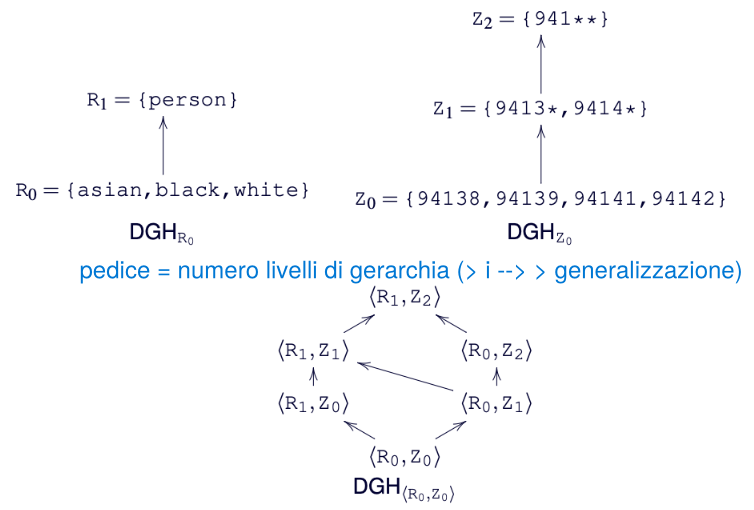
\includegraphics[width=1\linewidth]{images/domger.png}
\end{figure}


\subsubsection{Gerarchia di generalizzazione dei valori}

\begin{itemize}
    \item La relazione di generalizzazione dei valori \( \leq_V \) associa ad ogni valore nel dominio \( D_i \) un valore unico nel dominio \( D_j \), generalizzazione diretta di \( D_i \). 
    \item Questa relazione implica l'esistenza di una gerarchia di generalizzazione dei valori $ VGH_{D} $ per ciascun dominio \( D \).
    \item La $ VGH_{D} $ ha una struttura ad albero:
    \begin{itemize}
        \item \textbf{Foglie}: Rappresentano i valori nel dominio \( D \).
        \item \textbf{Radice}: È il valore più generale, situato nell'elemento massimo di $ DGH_{D} $.
    \end{itemize}
\end{itemize}

\newpage
\subsubsection{Esempio}

\begin{figure}[ht]
    \centering
    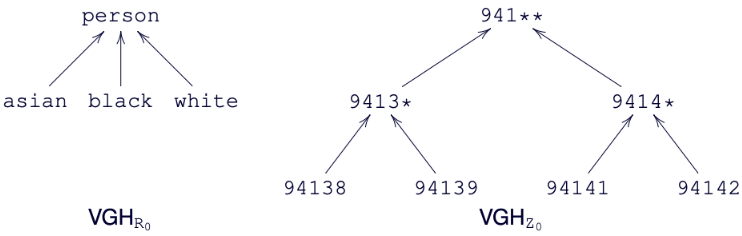
\includegraphics[width=1\linewidth]{images/valuegen.png}
\end{figure}

\subsubsection{Tabella generalizzata con soppressione}
Una tabella \( T_j \) è detta una generalizzazione (mediante soppressione di tuple) della tabella \( T_i \) (\( T_i \preceq T_j \)), se soddisfa le seguenti condizioni:

\begin{itemize}
    \item \( |T_j| \leq |T_i| \)
    \item Il dominio \( \text{dom}(A,T_j) \) di ogni attributo \( A \) in \( T_j \) è uguale o è una generalizzazione del dominio \( \text{dom}(A,T_i) \) dell'attributo \( A \) in \( T_i \).
    \item È possibile definire una funzione iniettiva che associa ogni tupla \( t_j \) in \( T_j \) con una tupla \( t_i \) in \( T_i \), tale che il valore di ogni attributo in \( t_j \) sia uguale o è una generalizzazione del valore dell'attributo corrispondente in \( t_i \).
\end{itemize}

\newpage
\subsubsection{\textit{k-minimal} generalization con soppressione}
Siano \( T_i(A_1, \ldots, A_n) \) e \( T_j(A_1, \ldots, A_n) \) due tabelle tali che \( T_i \preceq T_j \). Il \textbf{vettore di distanza} di \( T_j \) da \( T_i \) è definito come il vettore
\[
DV_{i,j} = [d_1, \ldots, d_n],
\] 
dove ogni \( d_z \) per \( z = 1, \ldots, n \) è la lunghezza del percorso unico tra \( dom(A_z, T_i) \) e \( dom(A_z, T_j) \) nella gerarchia di generalizzazione del dominio \( DGH_{D_z} \).
\\\\\\
Siano \( T_i \) e \( T_j \) due tabelle t.c. \( T_i \preceq T_j \), e sia \( MaxSup \) la soglia specificata di soppressione accettabile. La tabella \( T_j \) è detta una \textbf{generalizzazione k-minimale} della tabella \( T_i \) se e solo se:

\begin{enumerate}
    \item \( T_j \) soddisfa la k-anonymity garantendo la soppressione minima richiesta se per ogni tabella \( T_z \) che soddisfa la k-anonymity e t.c. \( T_i \preceq T_z \) e \( DV_{i,z} = DV_{i,j} \), allora deve valere \( |T_j| \geq |T_z| \).
    \item \( |T_i| \text{ - } |T_j| \leq MaxSup \) (non ho cancellato più del consentito)
    \item \( \forall T_z \text{ t.c. } T_i \preceq T_z \text{ e } T_z \text{ soddisfa le condizioni 1 e 2 } \Rightarrow \neg(DV_{i,z} < DV_{i,j}) \) $ \iff $ \(DV_{i,z} >= DV_{i,j} \)
\end{enumerate}

\subsubsection{Esempio}
$MaxSup = 2$
\begin{figure}[ht]
    \centering
    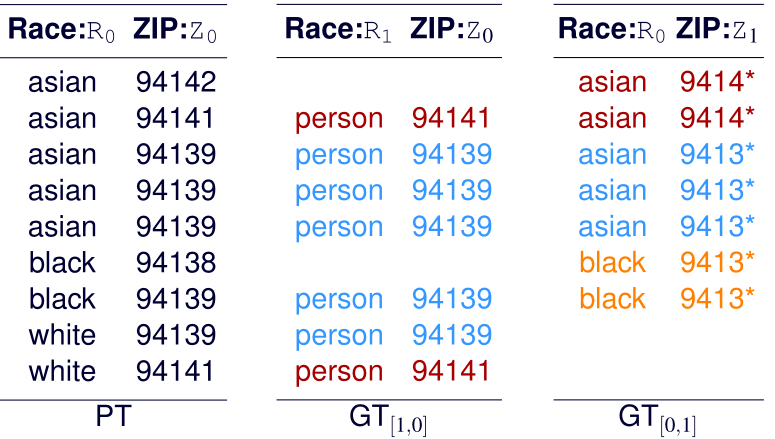
\includegraphics[width=1\linewidth]{images/k-minimal.png}
\end{figure}

\subsection{Computazione di una generalizzazione preferita}
Possono essere applicati diversi criteri di preferenza:
\begin{itemize}
    \item \textbf{Distanza assoluta minima:} minor numeri di passi di generalizzazione
    \item \textbf{Distanza relativa minima:} somma pesata, minimizza il mumero totali di passi relativi
    \item \textbf{Massima distribuzione:} maggior numero di tuple distinte
    \item \textbf{Minima soppressione} 
\end{itemize}

\subsection{Classificazione di tecniche per \textit{k-anonimity}}
Generalizzazione e soppressione possono essere applicate a diversi
livelli di granularità:
\begin{itemize}
    \item \textbf{Generalizzazione:} a livello di colonna o di cella
    \item \textbf{Soppressione:} a livello di riga, di colonna o di cella
\end{itemize}

\newpage
\section{Algoritmi per AG\_TS e AG\_}
\subsubsection{Computing a k-minimal solution}

\begin{itemize}
    \item Ogni percorso in $ DGH_{DT} $ rappresenta una strategia di generalizzazione per \( \text{PT} \)
    \item Chiamiamo \textit{locally minimal generalization} il nodo con indice minore in ogni percorso che soddisfa la \( k \)-anonymity
    \item Proprietà sfruttate dall'algoritmo:
    \begin{enumerate}
        \item Ogni \( k \)-minimal gen è localmente minima rispetto a un percorso, ma il contrario non è vero
        \item Salendo nella gerarchia, il \# di tuple da rimuovere per garantire la \( k \)-anonymity diminuisce
    \end{enumerate}
    \item Se non esiste una soluzione che garantisca la \( k \)-anonymity sopprimendo meno di \( \text{MaxSup} \) tuple all'altezza \( h \), non può esistere una soluzione con altezza inferiore a \( h \) che lo garantisca.
\end{itemize}

\noindent L'algoritmo adotta una ricerca binaria sul reticolo dei vettori distanza:

\begin{enumerate}
    \item Valuta le soluzioni all'altezza \( \left\lfloor \frac{h}{2} \right\rfloor \)
    \item Se esiste almeno una soluzione che soddisfa la \( k \)-anonymity:
    \begin{itemize}
        \item Valuta le soluzioni all'altezza \( \left\lfloor \frac{h}{4} \right\rfloor \)
    \end{itemize}
    \item Altrimenti valuta le soluzioni all'altezza \( \left\lfloor \frac{3h}{4} \right\rfloor \)
    \item Fino a quando l'algoritmo min(h) per la quale esiste un DV che soddisfa la \( k \)-anonymity
\end{enumerate}

\noindent Per ridurre il costo computazionale, l'algoritmo utilizza una matrice di vettori distanza.

\newpage
\subsubsection{k-Optimize algorithm}

\begin{itemize}
    \item Ordinare gli attributi nel quasi-identificatore (\textit{QI}) e i valori nei rispettivi domini.
    \item Associare un indice intero a ciascun valore del dominio, seguendo l'ordine definito.
\end{itemize}

\noindent Ad esempio:
\begin{center}
    \begin{tabular}{cc}
        \textbf{Race} & \textbf{ZIP} \\
        $\langle$[asian: 1] [black: 2] [white: 3]$\rangle$ & $\langle$[94138: 4] [94139: 5] [94141: 6] [94142: 7]$\rangle$ \\
    \end{tabular}
\end{center}

\begin{itemize}
    \item Una generalizzazione è l'unione dei singoli valori di indice.
    \item Il valore più basso in un dominio di attributi viene omesso. Ad esempio, \{6\} corrisponde a:
    \begin{itemize}
        \item \textbf{Race}: \{1\}, cioè: $\langle$[asian or black or white]$\rangle$
        \item \textbf{ZIP}: \{4, 6\}, cioè: $\langle$[94138 or 94139], [94141 or 94142]$\rangle$
    \end{itemize}
    \item L'ordine dei valori all'interno dei domini ha un impatto sulla generalizzazione.
\end{itemize}

\noindent L'algoritmo \textbf{k-Optimize} costruisce un \textbf{albero di enumerazione} per l'insieme degli indici $I$. \\
La radice dell'albero è l'insieme vuoto $\emptyset$, e i figli di ciascun nodo $n$ sono ottenuti aggiungendo un singolo elemento $i$ dell'insieme $I$, tale che $\forall i' \in n, i > i'$. 
Ogni nodo ha un \textbf{costo} che riflette la quantità di generalizzazione e soppressione associata all'anomizzazione rappresentata dal nodo. \\
L'algoritmo cerca l'anonimizzazione con il costo minimo attraverso una \textbf{visita dell'albero} tramite \textbf{ricerca in profondità}. 
Tuttavia, poiché l'albero ha $2^{|I|}$ nodi, la visita completa non è praticabile. Quindi viene adottata una strategia di \textbf{potatura (pruning)}:

\begin{itemize}
    \item Un nodo $n$ viene potato se nessuno dei suoi discendenti può fornire una soluzione ottimale.
    \item Questo si determina calcolando un \textbf{lb:limite inferiore} sul costo dei nodi nel sottoalbero radicato in $n$. 
    Se il limite inferiore è maggiore del miglior costo corrente, il nodo $n$ viene potato.
\end{itemize}

\newpage
\noindent \subsubsection{LO SPIEGHINO FATTO DA NOI:}
\begin{figure}[ht]
    \centering
    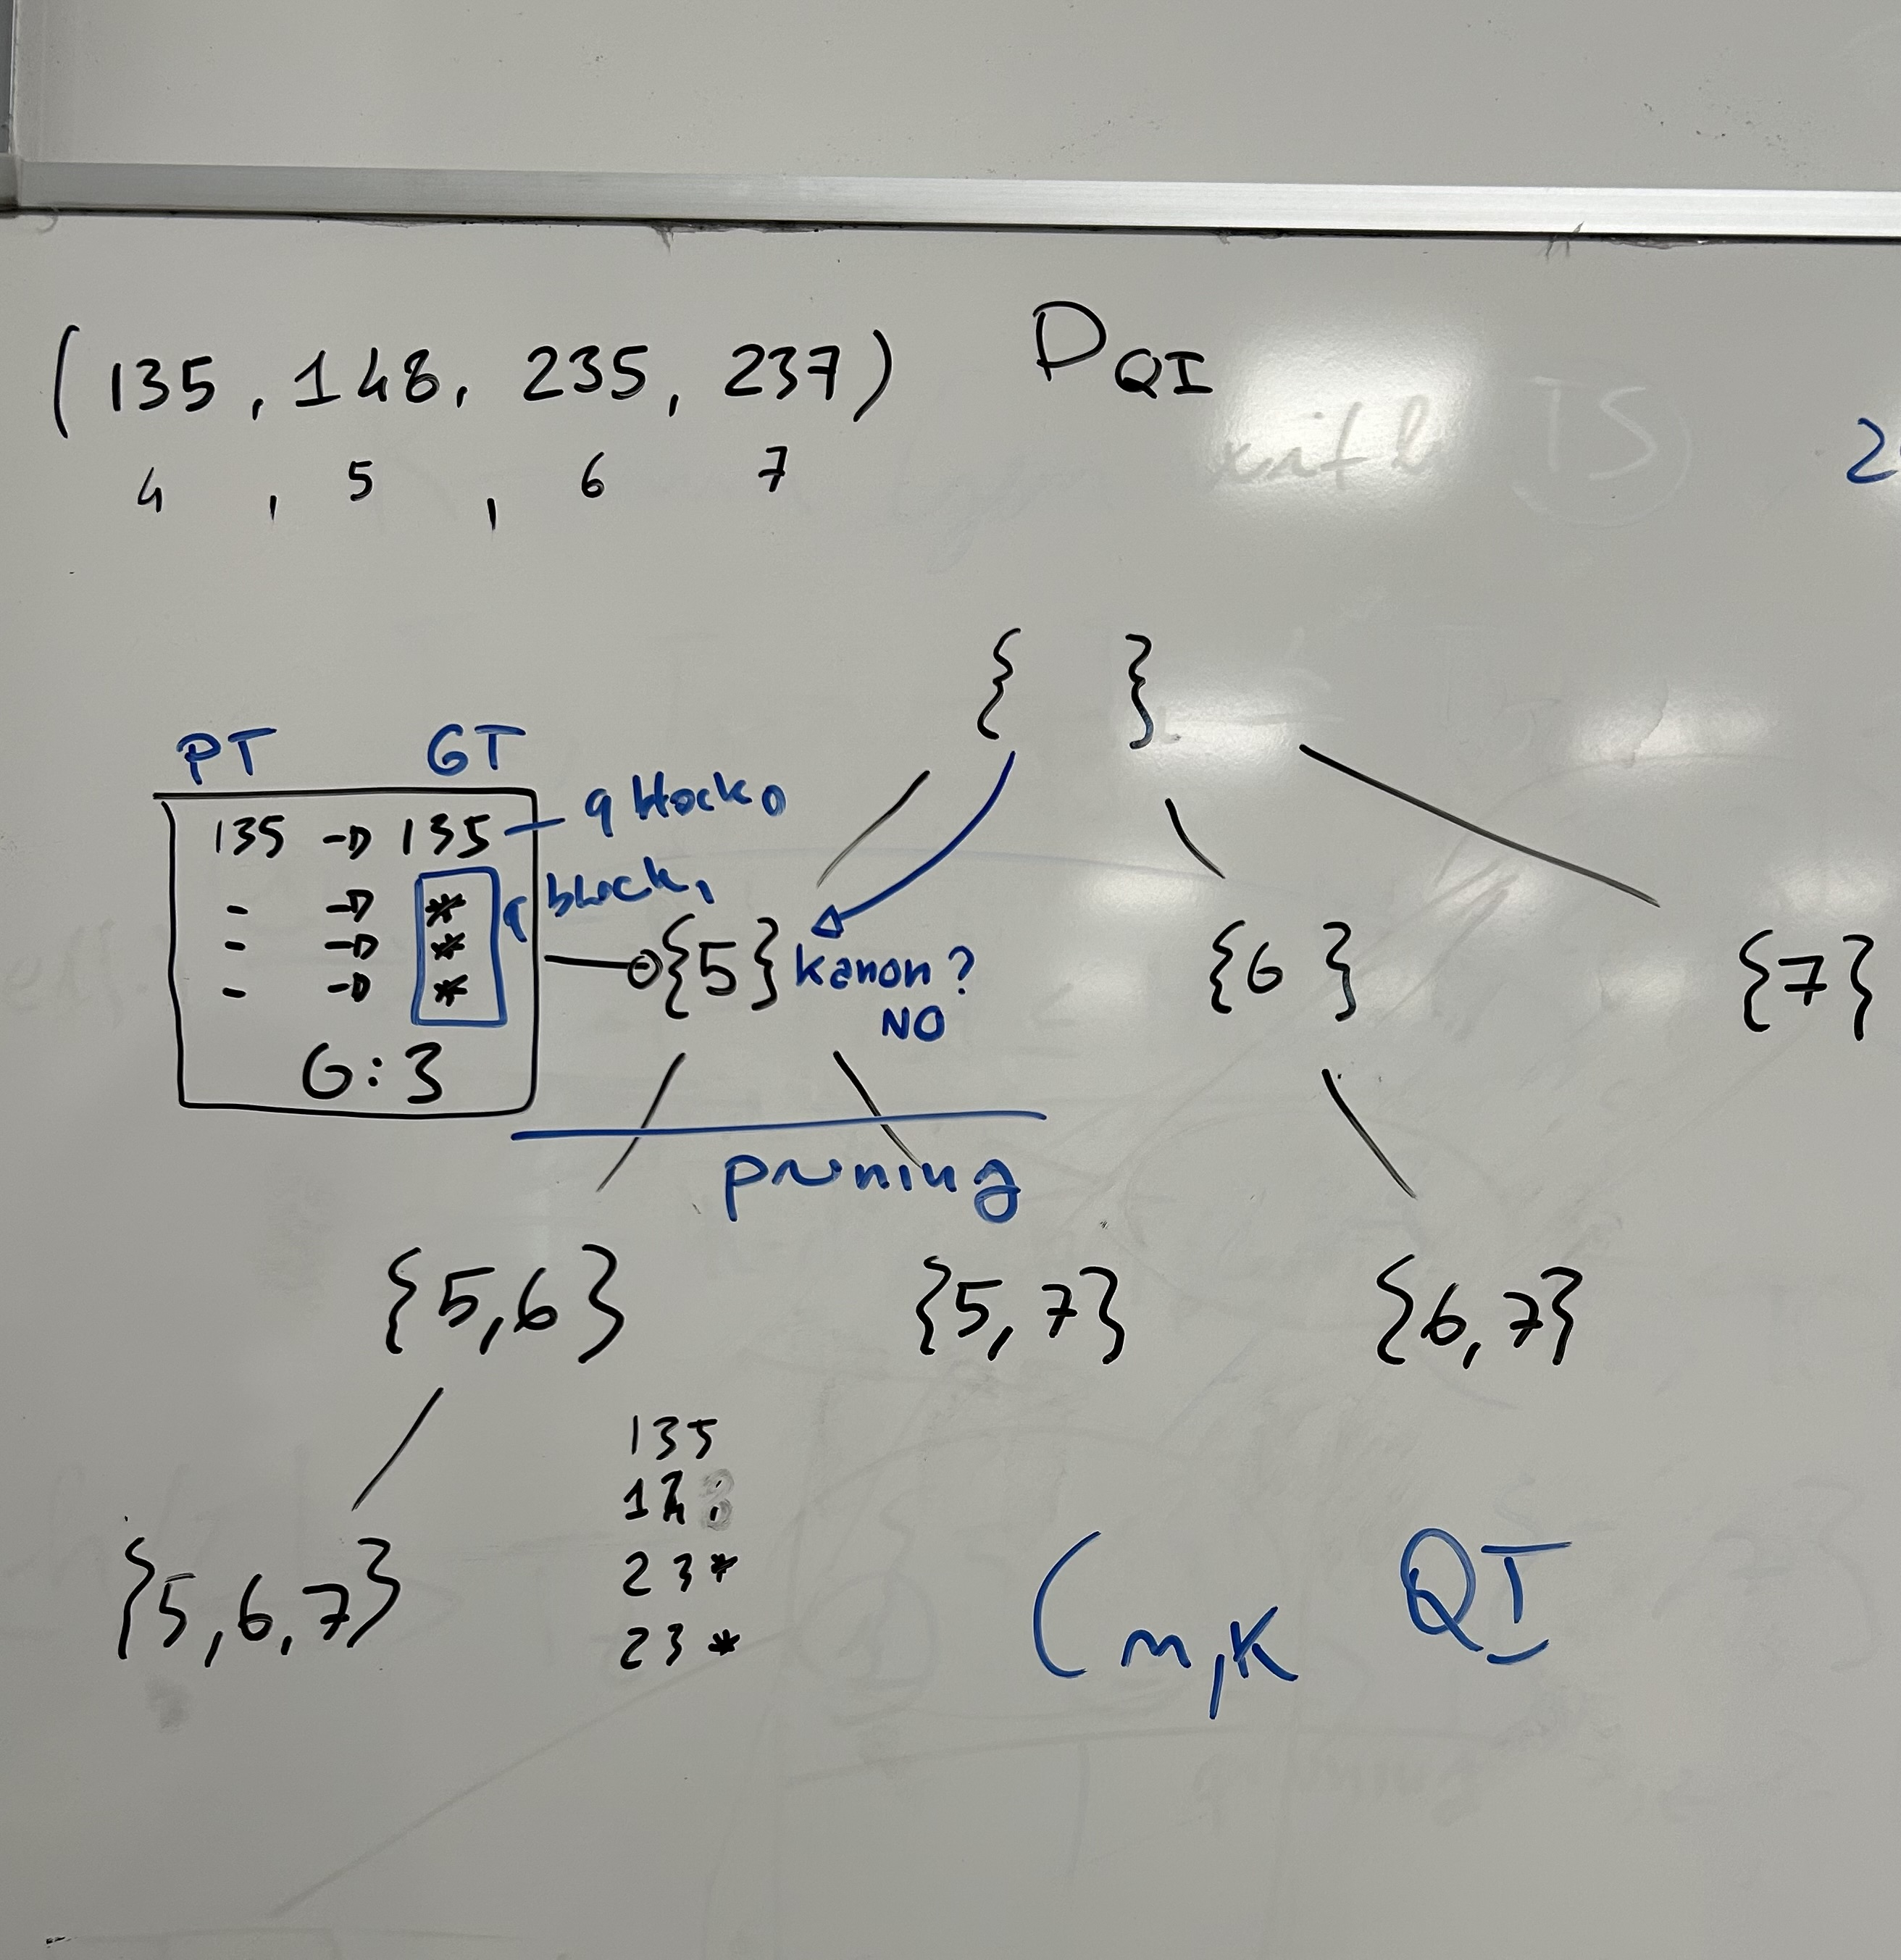
\includegraphics[width=1\linewidth]{images/foto k-optimize.jpg}
\end{figure}

\noindent L'algoritmo considera il dominio degli attributi del quasi-identifier e li indicizza globalmente ( indice numerico per ogni valore di ogni attributo, prendendo 
tutti i valori di tutti gli attributi).
A partire da questi ultimi fa un albero nel quale è presente ogni possibile partizionamento degli attributi, corrispondente alla creazione di cluster nella tabella. 
Ogni cluster avrà la propria generalizzazione e il proprio costo (per costo si intende quanti passi di generalizzaizone servono).
Ogni nodo del grafo corrisonde a un partizionamento e ogni figlio è un partizionamento successivo del padre (è un partizionamento della parte destra).
L'algoritmo, partendo dalla radice, esegue depth first search valutando per ogni nodo la k-anonimity della tabella: se la k-anonimity non è rispettata viene fatto \textbf{pruning}
su tutti i nodi figli e il depth firsy search continua sui nodi rimanenti.
Se, invece, k-anpnimity è rispettata depth first search continua verso i figli.
Viene infine scelta la soluzione che , soddisfando k-anonimity, ha il costo minore (minor numero di passi di generalizzazione).

\noindent Attenzione: se vediamo 6 significa che i cluster sono due: i numeri prima di 6, i numeri dopo 6 compreso il 6.
Se invece troviamo 5,6 allora i cluster saranno 3 $ \rightarrow $ 4 $ | $ 5 $ | $ 6 7

\noindent Es: a livello 5 i valori vengono divisi in due cluster, il primo con i valori prima di 5, il secondo con i valori dopo 5 (5 compreso).
In questa situazione ci troveremo con due cluster, il primo formato solo dal valore 135, il secondo con i valori 148, 235, 237.
Il valore 135 essendo da solo non necessita di nessun passo di generalizzazione, a differenza del secondo cluster che, avendo tre valori
completamente differenti andrà generalizzato al massimo.
L'algorito elabora una soluzione e verifica che rispetto alla nostra tabella, e al k richiesto, la soluzione sia k anonima.
Se è k anonima l'algoritmo va a controllare le soluzioni discendenti che potrebbero contenere soluzioni migliori,
nel caso non lo sia applica la tecnica del \textbf{pruning} e va a tagliare tutte le soluzioni sottostanti poichè non conterranno soluzione.


\newpage
\subsubsection{Incognito Algorithm}
L'algoritmo \textbf{Incognito} verifica \textbf{k-anonimity} con riferimento a un adeguato sottoinsieme del QI. \\ 
Esso adotta un approccio \textbf{bottom-up} per visitare le gerarchie di generalizzazione dei domini (DGHs). 
La condizione di k-anonimity rispetto a un sottoinsieme di QI è necessaria, ma non sufficiente per garantire la k-anonimity rispetto a tutto il QI. 
Il processo iterativo dell'algoritmo procede come segue:

\begin{itemize}
    \item \textbf{Iterazione 1}: si controlla la \textbf{k-anonimity} per ciascun attributo singolo in QI, scartando le generalizzazioni che non soddisfano la k-anonimity.
    \item \textbf{Iterazione 2}: si combinano le generalizzazioni rimanenti in coppie, verificando la \textbf{k-anonimity} per ciascuna coppia ottenuta. Scartando le coppie che non soddisfano la k-anonimity.
    \item \textbf{Iterazione n}: si considerano tutte le $n$-uple di attributi ottenuti dalle generalizzazioni che soddisfavano la k-anonimity nell'iterazione $i-1$, scartando le soluzioni che non la rispettano.
    \item $\ldots$
    \item \textbf{Iterazione $|$QI$|$}: restituisce il risultato finale, che rappresenta una generalizzazione che soddisfa la k-anonimity rispetto all'intero quasi-identificatore (QI).
\end{itemize}

\noindent L'algoritmo procede dunque costruendo progressivamente soluzioni, partendo da singoli attributi e combinandoli in gruppi via via più grandi fino a considerare tutti gli attributi del quasi-identificatore.

\newpage
\subsubsection{Esempio}
\begin{figure}[ht]
    \centering
    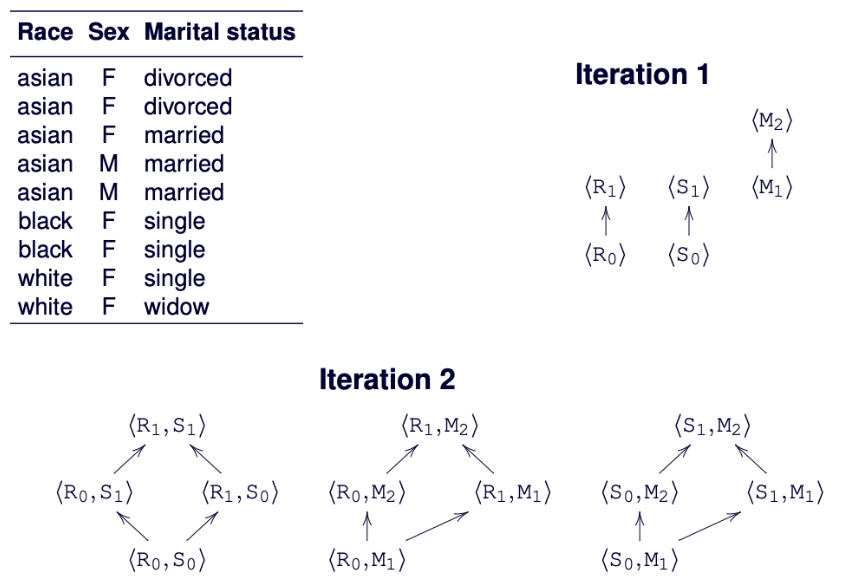
\includegraphics[width=1\linewidth]{images/incognito.png}
\end{figure}
In questo caso vogliamo un $k=2$; per questa ragione l'ultima riga della tabella 
(\textit{widow}) viene scartato poiché c'è solo un rispondente per tale valore.

È per questo che $M_0$ non è presente; viene sopppresso e si parte da $M_1$.


\newpage
\section{Algoritmi per \_CS e CG\_}

\subsection{Mondrian Multidimensional Algorithm}
L'algoritmo \textbf{Mondrian Multidimensional} si basa su una rappresentazione spaziale delle tuple e dei quasi-identificatori:

\begin{itemize}
    \item Ogni attributo nel quasi-identificatore (\textbf{QI}) rappresenta una dimensione.
    \item Ogni tupla nel set di dati privati (\textbf{PT}) rappresenta un punto nello spazio definito da \textbf{QI}.
    \item Le tuple con lo stesso valore di \textbf{QI} sono rappresentate assegnando una molteplicità ai punti.
    \item Lo spazio multidimensionale viene partizionato dividendo le dimensioni in modo tale che ogni area contenga almeno $k$ occorrenze di valori dei punti. 
    \item Tutti i punti in una regione vengono generalizzati a un valore unico.
    \item Le tuple corrispondenti sono sostituite dalla generalizzazione calcolata.
\end{itemize}

\noindent L'algoritmo Mondrian è flessibile e può operare:
\begin{itemize}
    \item \textbf{Su un numero diverso di attributi:} 
    \begin{itemize}
        \item \textit{Single or Multi-dimension}.
    \end{itemize}
    \item \textbf{Con diverse strategie di generalizzazione:}
    \begin{itemize}
        \item \textit{Global or Local recoding}: colonna o cella.
    \end{itemize}
    \item \textbf{Con diverse strategie di partizionamento:} 
    \begin{itemize}
        \item \textit{Strict or Relaxed partitioning}: senza o con possibili sovrapposizioni (con \textit{relaxed} due occorrenze uguali possono appartenere a cluster diversi).
    \end{itemize}
    \item \textbf{Utilizzando metriche diverse per determinare come dividere ogni dimensione.}
\end{itemize}

\newpage
\subsubsection{Esempio}
Wished $k = 3$
\begin{figure}[ht]
    \centering
    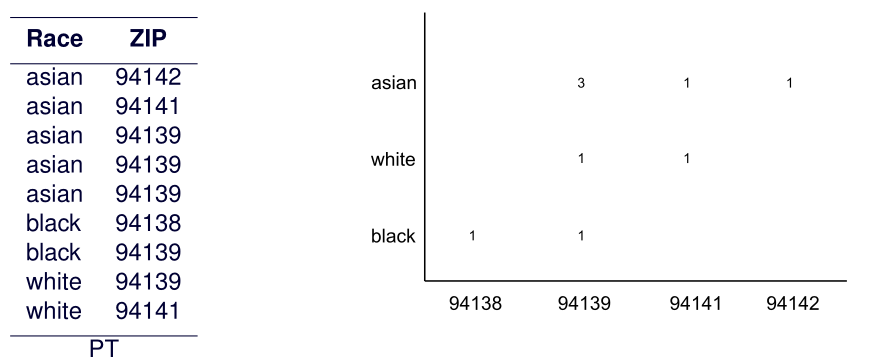
\includegraphics[width=1\linewidth]{images/mondrian1.png}
\end{figure}

\noindent Ogni tupla è un punto nello spazio; in questo caso ogni taglio deve rispettare $k=3$.
C'è un'idea di ordinamento dei valori; con i numeri ha senso con altri valori è forzato.

Le tuple vengono divise in cluster; le tuple di ogni cluster vengono rese uguali generalizzandole.

\begin{figure}[ht]
    \centering
    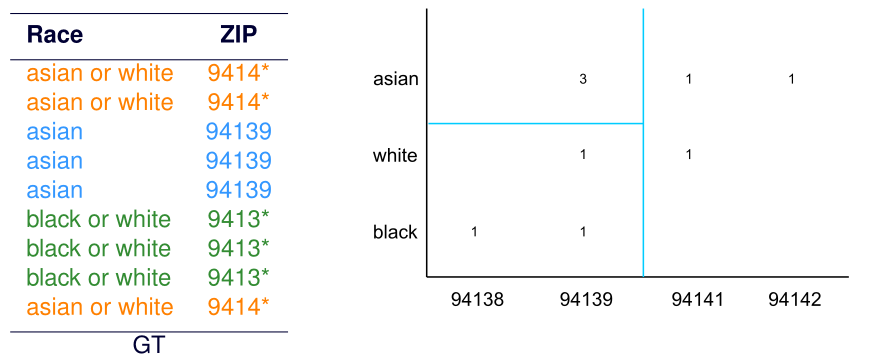
\includegraphics[width=1\linewidth]{images/mondrian2.png}
\end{figure}

\subsection{k-anonymity Revisited}
La \textbf{k-anonymity} cambia a seconda del livello di generalizzazione applicato:

\begin{itemize}
    \item \textbf{AG:} Ogni n-upla di quasi-identificatori deve apparire almeno $k$ volte.
    \item \textbf{CG:} La condizione di avere almeno $k$ occorrenze è sufficiente ma non necessaria. È possibile utilizzare un requisito meno restrittivo:
    \begin{enumerate}
        \item Per ogni sequenza di valori $pt$ in $\mathit{PT[QI]}$, ci devono essere almeno $k$ tuple in $\mathit{GT[QI]}$ che contengono una sequenza di valori che generalizzano $pt$.
        \item Per ogni sequenza di valori $t$ in $\mathit{GT[QI]}$, ci devono essere almeno $k$ tuple in $\mathit{PT[QI]}$ che contengono una sequenza di valori per cui $t$ è una generalizzazione.
    \end{enumerate}
\end{itemize}

\noindent La generalizzazione a livello di cella permette una maggiore flessibilità rispetto alla gen a livello di attributo.

\section{Attribute disclosure}

La \textit{k-anonimity} è vulnerabile a diversi attacchi.
\begin{itemize}
    \item \textbf{Omogeneità dei valori di attributi sensibili:} se tutti gli appartenenti ad un gruppo
    hanno la stessa informazione sensibile, mi basta conoscere che appartieni a quel gruppo per sapere che hai quella informazione sensibile
    \begin{figure}[ht]
        \centering
        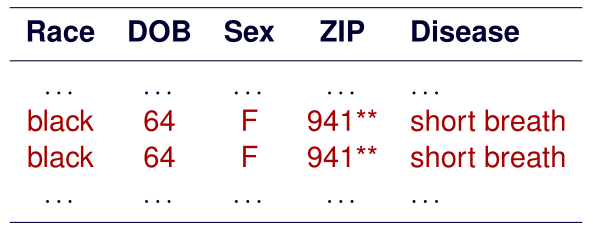
\includegraphics[width=0.5\linewidth]{images/omogen.png}
    \end{figure}
    \item \textbf{Conoscenza pregressa:} è conoscenza a livello di istanza che posso avere e mi permette di scartare alcune possibilità; nella figura, se
    so che corri due ore al giorno deduco che non hai il fiato corto.
    \begin{figure}[ht]
        \centering
        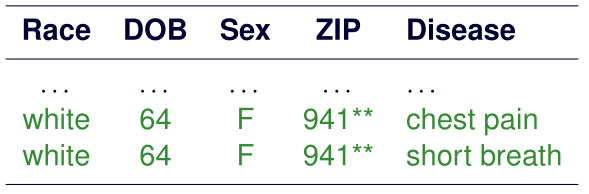
\includegraphics[width=0.5\linewidth]{images/back.know.png}
    \end{figure}
\end{itemize}

\subsection{\texorpdfstring{$\ell$}{l}-Diversity}
Definiamo un \textit{q-block} come un gruppo di tuple con lo stesso \textit{quasi-identifier};
diciamo che un \textit{q-block} è \texorpdfstring{$\ell$}{l}-diverse se contiene almeno
\texorpdfstring{$\ell$}{l} valori \textbf{differenti} e \textit{\textbf{ben rappresentati}} per l'attributo sensibile.

Questo implica che un attaccante deve eliminare almeno \texorpdfstring{$\ell$}{l}$-1$ valori 
possibili per inferire un valore sensibile di un rispondente.

Una tabella è \texorpdfstring{$\ell$}{l}-diverse se tutti i suoi \textit{q-block} sono
\texorpdfstring{$\ell$}{l}-diverse; questo implica che:
\begin{itemize}
    \item l'attacco di omogeneità non è possibile
    \item l'attacco di conoscenza pregressa è più difficile (devo eliminare \texorpdfstring{$\ell$}{l}-1 possibilità)
\end{itemize}

\texorpdfstring{$\ell$}{l}-diversity può lasciare spazio a degli attacchi basati sulla distribuzione 
dei valori all'interno dei \textit{q-block}.

\subsubsection{Skewness attack (attacco di distorsione)}
Avviene quando un  \textit{q-block} ha una distribuzione diversa da quella del mondo reale;
quando faccio i gruppi devo sia avere dei valori diversi che dei valori simili a quelli attesi.

\subsubsection{Attacco di similarità}
Avviene quando un \textit{q-block} contiene dei valori che sono diversi ma semanticamente 
simili (ad esempio, ulcera allo stomaco/gastrite).

\subsubsection{\textit{t}-closeness}
Diciamo che un \textit{q-block} rispetta \textit{t-closeness} se la distanza 
tra la distribuzione dei valori degli attributi sensibili nel \textit{q-block} 
e quella della popolazione di riferimento è minore di \textit{t}.

Una tabella rispetta \textit{t-closeness} se tutti i suoi \textit{q-blocks}
rispettano \textit{t-closeness}.

\subsection{Tipi di conoscenza pregressa}
Le conoscenze possono riguardare:
\begin{itemize}
    \item l'individuo target
    \item altri individui, il che potrebbe comunque rivelare informazioni sensibili
    \item famiglie di valori uguali, come informazioni genomiche che collegano un gruppo di persone.
\end{itemize}

\subsection{Rilasci multipli}
I dati potrebbe essere soggetti a rilasci multipli, come aggiornamenti o pubblicazioni 
ricorrenti.
Con il rilascio multiplo di multiplo ci si espone ad attacchi di intersezione, 

\subsection{\textit{m-invariance}}
Per affrontare il problema dei rilasci longitudinali, una sequenza $T_1, ..., T_n$ di tabelle di microdati rilasciate soddisfa la proprietà di \textit{m-invariance} se:

\begin{itemize}
    \item ogni classe di equivalenza contiene almeno $m$ tuple;
    \item nessun valore sensibile appare più di una volta in ciascuna classe di equivalenza;
    \item per ogni tupla $t$, le classi di equivalenza a cui appartiene $t$ nella sequenza sono caratterizzate dallo stesso insieme di valori sensibili.
\end{itemize}

\noindent Ciò implica che la correlazione delle tuple in $T_1, ..., T_n$ non permette a un destinatario malevolo di associare meno di $m$ valori sensibili differenti a ciascun rispondente.

\section{\textit{k-anonimity} in altre applicazioni}

\subsection{Social Networks}
In una rete sociale ciò che ti può rendere peculiare è il numero
di connessioni che hai (esempio influencer); si cerca di avere ogni nodo 
uguale ad almeno altri $k$, dove $k$ è il grado di protezione che voglio ottenere.

Per fare questo si è possibile sopprimere o aggiungere archi.


\subsection{Data Mining}
Il \textit{k-anonymous data mining} mira a garantire che i risultati del data mining non violino i requisiti di \textit{k-anonymity} sui dati originali.
Alcuni esempi di tecniche per compromettere la k-anonymity sfruttando il data mining includono:

\begin{itemize}
    \item \textbf{Association Rule Mining}: tecniche per trovare regole di associazione possono compromettere la k-anonymity.
    \item \textbf{Classification Mining}: tecniche di classificazione possono portare a minacce per la privacy.
\end{itemize}

\subsection{Location-Based Services}
Bisogna preocupparsi del fatto che la locazione di un individuo potrebbe 
rivelare la sua identità. Così come si generalizza il valore dei dati per aumentare
il numero degli utenti ed avere più incertezza, lo stesso viene fatto con
la posizione.

\noindent \\Si può adottare il concetto di \textit{k-anonimity} come segue:
\begin{itemize}
    \item Considerare solo le aree che contengono almeno $k$ individui
    \item Ingrandire l'area per includere almeno altri $k-1$ utenti (\textit{k-anonymity})
    \item Obfuscazione delle aree (\textit{location privacy}) per ridurre la precisione o la confidenza dei dati; magari non si può semplicemente ingrandire perché l'utente si troverebbe al centro
    \item Protezione del percorso degli utenti (\textit{trajectory privacy}) tramite modifica delle traiettorie
\end{itemize}

\section{Privacy Sintattica e Semantica}
\begin{itemize}
    \item \textbf{Syntactic Privacy:}
    le definizioni di privacy sintattiche misurano il grado di protezione di una persona nei dati con un valore numerico. 
    
    Ad esempio:
    \begin{itemize}
        \item Ogni rilascio di dati deve essere indistinguibilmente associato ad almeno un certo numero di individui nella popolazione.
    \end{itemize}

    \item \textbf{Semantic Privacy:}
    le definizioni di privacy semantiche soddisfano un requisito di privacy semantico. 
    
    Ad esempio:
    \begin{itemize}
        \item Il risultato di un'analisi eseguita su un dataset rilasciato non deve essere influenzato dalla presenza o assenza di una singola tupla nel dataset.
    \end{itemize}
\end{itemize}

\section{Differential Privacy}
La \textit{Differential Privacy} mira a prevenire che un attaccante sia in grado di stabilire
la presenza o l'assenza di un individuo in un dataset. È un tipo di \textit{semantic privacy}.
\subsubsection{Definizione informale}
La distribuzione della probabilità sui dati pubblicati deve essere \textit{essenzialmente la stessa}
indipendentemente dal fatto che un individuo sia incluso o meno nel dataset.

\begin{figure}[ht]
    \centering
    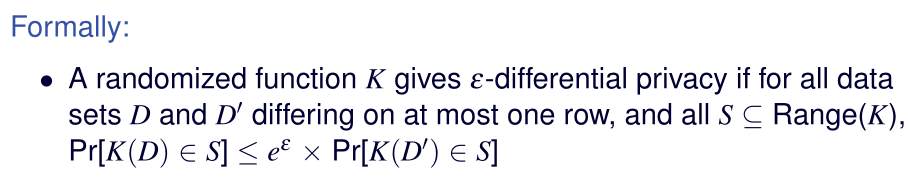
\includegraphics[width=0.85\linewidth]{images/diff.png}
\end{figure}

L'obiettivo della funzione randomizzata è quello di aggiungere rumore;
c'è da tenere in considerazione il \textit{trade-off} tra introduzione del rumore 
e utilizzabilità dei dati. 

\noindent $e^\epsilon$ indica il \textit{privacy budget}, che diminuisce man mano che il dataset 
viene interrogato; quando si esaurisce non si potrà più interrogare quel dataset. 
\begin{itemize}
    \item $\epsilon = 0 \rightarrow$ non mi dice niente, risposta qualsiasi
    \item $\epsilon = 1 \rightarrow$ dato preciso, utile ma poca privacy
    \item $0 < \epsilon < 1 \rightarrow$ c'è del rumore ma ho dati utili
\end{itemize}

La \textit{differential privacy} può essere applicata in due scenari:
\begin{itemize}
    \item \textbf{Interattivo:} valutazione a run-time delle query (statistical DBMS)
    \item \textbf{Non interattivo:} rilascio di tabelle pre-computate (statistical data)
\end{itemize}

Viene rinforzata aggiungendo del rumore casuale, a discapito della veridicità dei dati.

\subsubsection{\textit{k-anonimity} vs \textit{differential privacy}}
\begin{itemize}
    \item \textbf{\textit{k-anonimity}}
    \begin{itemize}
        \item \textcolor{darkgreen}{rappresenta bene il mondo reale}
        \item \textcolor{red}{protezione non completa}
    \end{itemize}
    \item \textbf{\textit{differential privacy}}
    \begin{itemize}
        \item \textcolor{darkgreen}{garantisce una miglior protezione}
        \item \textcolor{red}{non garantisce protezione completa, è più complicato fare \textit{enforce}}
    \end{itemize}
\end{itemize}


\chapter{Alcuni esempi di altri problemi di privacy}
\section{Distribuzione di valori sensibili}
Riesco ad inferire informazioni non dalla singola tupla, ma dall'insieme di tuple.
\subsubsection{Esempio: Soldiers' Medical Records}
\begin{itemize}
    \item I record individuali non sono sensibili.
    \item La distribuzione dell'età dei soldati in una località può indicare il tipo di località:
    \begin{itemize}
        \item Soldati giovani suggeriscono tipicamente un campo di addestramento.
        \item Funzionari più anziani indicano un quartier generale.
    \end{itemize}
\end{itemize}

\section{Dati del genoma}
Le informazioni genomiche presentano opportunità in medicina ma sollevano anche diversi problemi di privacy:
\begin{itemize}
    \item Il genoma umano può identificare il suo proprietario
    \item Contiene informazioni sensibili sulla provenienza etnica, predisposizione a malattie e altri tratti fenotipici
    \item I dati genomici possono rivelare informazioni sui parenti e sui discendenti sulla base del genoma (non solo tua)
\end{itemize}

\section{Social Media}
Le nostre attività sui social media e i "like" possono rivelare informazioni sensibili. 

È importante notare che i social media condividono frequentemente i nostri dati con terze parti, come inserzionisti e aziende di analisi, il che può portare a violazioni della privacy.

\section{Dati Biometrici}
La privacy dei dati biometrici solleva ulteriori preoccupazioni; sono sistemi in grado di identificare gli utenti 
senza il loro consenso.



\end{document}